\documentclass{article}
\usepackage[utf8]{inputenc}
\usepackage{hyperref}
\hypersetup{
    colorlinks=true,
    linkcolor=blue,
    filecolor=magenta,      
    urlcolor=cyan,
}
 
\urlstyle{same}

\usepackage{graphicx}

\newcommand{\chapsubhead}[1]{{\Large #1 \vspace{2ex}}}
\newcommand{\chaptype}[1]{{\Large \itshape (#1) \vspace{2ex}}}
\title{Learning Journal}
\author{Lauren Franks }
\date{FOAR705}

\begin{document}

\maketitle
\tableofcontents


\section{Data Organization in Spreadsheets for Social Scientists}
\addcontentsline{toc}{section}{1.1 Formatting data tables in spreadsheets}
\chapsubhead{1.1 Formatting data tables in spreadsheets}\\
\textbf{Exercise 1:}\newline

Objective: To clean up messy data sheets using Open Refine\\
Action: Opened OpenRefine software, uploaded SAFI Messy data set and created new project.\\
Error: Realised that I lack sufficient expertise in OpenRefine to proceed.\\ 
Result: Returned to excel.\\

Objective: Identify problems with data set\\
Action: Reviewed data carpentry literature for guidance and identified following errors:
Colourful cells, misspellings, inconsistent recording styles, empty cells where there should be zeros, uses multiple sheets, uses multiple tables, uses symbolic formatting to show information, uses white space.\\
Result: successful identification of errors.\newline

Objective: To clean up Mozambique data according to previously identified problems
Actions:
\begin{enumerate}
\item Created new sheet in Excel and copy pasted data for Mozambique
\item Added new column for ‘inc barn’ and removed coloured cell
\item Moved ‘livestock’ and ‘plots’ graph to separate columns adjacent to dwelling graph
\item Created four separate columns for poultry, oxen, cows and goats
\item Created separate columns for ‘water use’ and ‘water use summer only’
\end{enumerate}
Errors identified in data:
\begin{itemize}
\item Key id 6 amount/type of livestock is not clear in original data set
\item Meaning of ‘look after cows’ column is unclear in original data set as it seems to directly contradict information in original ‘livestock owned and numbers’ column which suggests that key id 2, 4, 5, and 9 all have cows
\item Both livestock and plot data from key id 10 is omitted entirely from original data set
\end{itemize}

Result:
Data is much clearer to read, however errors listed above are unable to be sufficiently addressed without further information from original researchers. \\

Objective: To clean up Tanzania data according to previously identified problems\\
Action: Copy pasted data for Tanziania into cleaned data tab on spreadsheet\\
Result: Success\\
Action: Created new column for the country to differentiate between key id locations in Tanzania and Mozambique\\
Result: Success\\
Action: Created new column for ‘inc cowshed’\\
Result: Success\\

Errors identified in data:
\begin{itemize}
\item Unsure if ‘burntbricks’ and ‘sunbricks’ refer to the same value
\end{itemize}
\begin{itemize}
\item Key id 16 says it has 1 poultry, 1 oxen and 1 goat and yet a total of 4 livestock
\item Key id 18 says it have a total of 1 livestock but does not list which kind
\item No livestock data for key id 20
\item No data for plots
\end{itemize}
Solutions:
\begin{itemize}
\item Added column ‘livestock unspecified’  
\item I have opted to leave spaces black where data is unavailable as this is the best null value according to the Data Carpentry website.
\end{itemize}
Results:
\begin{itemize}
\item Saved sheet as a new excel spreadsheet called 'SAFI messy fixed Franks2019'
\item Data is much clearer to read, however there remain some missing values as I was unable to deduce the answers from the available data. To fully complete data set would require discussion with original researchers. 
\end{itemize}

\textbf{Exercise 2:}\\
Objective: Identify what types of metadata should be recorded from the regarding the data set.\\
Action: I discussed with Ellen about what types of metadata should be recorded. As per the Data Carpentry website, we concluded that some types of metadata that should be recorded and made available with the data are:
\begin{itemize}
\item the exact wording of questions used in the interviews (if interviews were structured) or general prompts used (if interviews were semi-structured)
\item a description of the type of data allowed in each column (e.g. the allowed range for numerical data with a restricted range, a list of allowed options for categorical variables, whether data in a numerical column should be continuous or discrete)
\item definitions of any categorical variables (e.g. definitions of “burntbricks” and “sunbricks”) 
\item definitions of what was counted as a “room”, a “plot”, etc. (e.g. was there a minimum size)
\end{itemize}

\textbf{Two examples of problem data produced in politics and international relations:}
\begin{enumerate}
\item Adam Smith, 18th century philosopher and arguably the founder of modern economic theory, wrote that barter was a precursor to money. Despite there being no evidence for this claim it appears in many politics and economics textbooks. A similar false claim is ‘trickle down economics’, this flawed idea is used as data to back up flawed arguments.
\item 	Data bias in policing is a political issue. \newline
\end{enumerate}

\addcontentsline{toc}{section}{1.2 Dates as data}
\chapsubhead{1.2 Dates as data}\\
\textbf{Exercise 1:}\newline 
Objective: To separate dates into components in a spread sheet\\
Action:	Download and open dates excel file\\
Result: Success\\
Action: Created 3 new columns for day, month and year and separated dates into those columns\\ 
Result: Success\\
Action: Tried to used the automated functions on excel to input the days.\\
Error: It put a whole date in instead of the day.\\
Solution: I chose to enter the days manually into excel as there weren’t too many, however, this is not an acceptable solution for the future and I will need to revisit this.\\

\addcontentsline{toc}{section}{1.3 Quality assurance}
\chapsubhead{1.3 Quality assurance}\newline
Objective: Apply data validation rule to restrict data to a specific numeric range\\
Action: followed instructions on website and didn’t have any issues.\\
Objective: Save excel file as csv file\\
Error: Cannot save csv with multiple worksheets\\
Solution: Saved both sheets as separate csv files.\\

\section{The Unix Shell}
\addcontentsline{toc}{section}{2.1 Introducing the Shell}
\chapsubhead{2.1 Introducing the Shell}\\
Objective: Use GitBash to list content of directory\\
Action: Typed ls\\ 
Result: Successfully listed directory\\

\addcontentsline{toc}{section}{2.2 Navigating Files and Directories}
\noindent\chapsubhead{2.2 Navigating Files and Directories}

Objective: Learn to navigate using the shell\\
Action: Used ls (list directory contents), cd (change directory), and pwd (tells you where you are) \\
Result: It worked.\\

\section{OpenRefine}

To open Open Refine, open openrefine.exe and then go to http://127.0.0.1:3333/ (may need to wait a little while after opening the .exe file for the web link to work)\newline 

\addcontentsline{toc}{section}{3.1 Working with OpenRefine}
\chapsubhead{3.1 Working with OpenRefine}\\
Objective: Apply filters to view facet groups in Open Refine\\
Action: Clicked down arrow on village column and chose Facet, Text facet. \\
Result: Success. Was able to filter and see unique value in the village column along with a number representing how many times that value occurs in the column.\\
Errors: None. \newline

Objective: Identify problems with data set?\\
Action: Reviewed data using facet filters as above.\\
Result: Many misspellings including ‘Chirdozo’ which should be ‘Chirodzo’, ‘Ruca’ which should be ‘Ruaca’. \newline

Objective: Use faceting to find how many different interview\textunderscore date values are in the survey results.\\
Action: Clicked down arrow on interview\textunderscore date column and chose Facet, Text facet.\\
Result: Success, panel on left shows there are 19 choices (values).\newline

Objective: Convert column from text to date.\\
Action: Clicked down arrow on interview\textunderscore date column, Edit cells, Common transforms, To date.\\
Result: Success, changed to date value. You can see that the data was collected in 2016.\newline

Objective: Use ‘clustering’ to identify possible typing errors/inconsistencies. \\
Action: Clicked cluster on the village Text Facet, chose key collision method and metaphone3 keying function which identified two clusters. Ticked the Merge? box beside each one, Merge Selected and Recluster.\\
Result: Success. \newline

Objective: Correct errors in data set that clustering did not fix.\\
Action: Hovered over ‘Ruaca-Nhamuenda’,  Edit, and changed to Ruaca.\\ Hovered over ‘Chirdozo’ , Edit and changed to ‘Chirodzo’. 
Result: Success, I now have only four clusters. \newline

Objective: Remove single quote marks ( ‘ ), right square brackets ( ] ) and spaces from the items\textunderscore owned column.\\
Action: Clicked down arrow on items \textunderscoreowned column. Chose Edit Cells ,  Transform... Entered value.replace("]", "")  into the expression box and clicked OK. Repeated with value.replace("’", "")  and value.replace(" ", "") \\
Result: Success, items\textunderscore owned column is now separated by semicolons.\newline
  

Objective: Determine what the two most commonly owned items are.\\
Action: Clicked the down arrow on items\textunderscore owned column. Chose Facet ,  Custom text facet... Typed type value.split(";") in the expression box and clicked OK. On new text facet box clicked Sort by: count.\\
Result: Success, two most commonly owned items are mobile phones and radios (86 each).\newline


Objective: Clean up and customise months\textunderscore lack\textunderscore food column to determine which month farmers were most likely to lack food.\\
Action: Clicked down arrow on months\textunderscore lack\textunderscore food column. Chose Edit Cells ,  Transform... Entered value.replace("[", "").replace("]", "").replace(" ", "").replace("'", "")  into the expression box and clicked OK.  Clicked the down arrow on months\textunderscore lack\textunderscore food column. Chose Facet ,  Custom text facet... Typed type value.split(";") in the expression box and clicked OK. On new text facet box clicked Sort by: count.\\
Result: Success, November is when farmers are most likely to lack food (71).\newline

Objective: Perform same clean up steps on months\textunderscore no\textunderscore water, liv \textunderscoreowned, res\textunderscore change, and no\textunderscore food\textunderscore mitigation columns.\\
Action: Clicked down arrow on each of the columns in turn. Chose Edit Cells ,  Transform... Went to History Tab, clicked Reuse on previous command cluster,  Ok.\\
Result: Success, using history tab much faster than entering commands individually.\newline


Objective: Learn how to use undo/redo functions.\\
Action: Clicked Undo / Redo on left side of scree, went back a few steps and saw when columns still contained special characters. Clicked on some steps to undo/redo actions.\\
Result: Success. \newline

Objective: Remove blank characters from beginning and end of entries.\\
Action: Created new text facet by clicking down arrow on respondent\textunderscore wall\textunderscore type column, then Facet, Text facet. Clicked down arrow on respondent\textunderscore wall\textunderscore type column, clicked Edit cells,  Common transforms, Trim leading and trailing whitespace.\\
Result: Success, there are now only four choices in the text facet.\newline

\addcontentsline{toc}{section}{3.2 Filtering and sorting with OpenRefine}
\noindent\chapsubhead{3.2 Filtering and sorting with OpenRefine}\\
Objective: Use filtering to work on only a subset of data.\\
Action: Clicked down arrow on respondent\textunderscore roof\textunderscore type ,  Text filter. Typed mabat into the  respondent\textunderscore roof\textunderscore type facet and pressed enter. Change the view at the top of page to Show 50 rows. Created new text facet by clicking down arrow on respondent\textunderscore roof\textunderscore type column, then Facet, Text facet.\\
Result: Success, roof types show mabatipitched and mabatisloping. To restrict to only one of these values I could include more letters in the filter.\newline

Objective: Use include/exclude to select only one of these roof types (either mabatipitched or mabatisloping)\\
Action: Hovered over ‘mabatipitched’ on the text facet on the left side and clicked Include.\\
Result: Success, I am now only seeing rows with mabatisloping values. I can also do the same steps to exclude one or the other.\newline

Objective: Use sort function to sort data by gps\textunderscore Altitude\\
Action: Clicked down arrow on gps:Altitude column, Sort... ,  numbers and selected smallest first. \\
Result: Success, the zero value on many of the entries suggests that the data is missing. \newline

Objective: Use sorting of GPS data to determine which village ‘49’ is.\\
Action: Sorted gps\textunderscore Longitude and gps\textunderscore Lattitude as a number with the largest first. Clicked down arrow on village column, clicked Edit column ,  Move column to end. Scrolled down to village 49. \\
Result: Success, it belongs to a cluster of interviews in Chirodzo.\newline

\addcontentsline{toc}{section}{3.3 Examining numbers in OpenRefine}
\noindent\chapsubhead{3.3 Examining numbers in OpenRefine}

Objective: Transform text values to number values.\\
Action: Clicked down arrow on years\textunderscore farm column, \textgreater Edit cells  \textgreater Common transforms… \textgreater To number.\\
Result: Success, values changed from left-justified to right-justified, and black to green in colour.\newline

Objective: Transform no\textunderscore members, yrs \textunderscore liv, and buildings\textunderscore in\textunderscore compound, from text to numbers.\\
Action: As above, clicked down arrow on columns, \textgreater Edit cells  \textgreater Common transforms… \textgreater To number.\\
Result: Success. Unable to transform columns without numeric values into numbers, such as the village column.\newline

Objective: Find non-number values or blanks in a column.\\
Action: Replaced a number in buildings\textunderscore in\textunderscore compound with `abc’. Created a numeric facet using down arrow. Unchecked numeric checkbox on facet to display the row I changed to ‘`abc’.\\
Result: Successfully found non-number value.\newline

\addcontentsline{toc}{section}{3.4 Using Scripts}
\noindent\chapsubhead{3.4 Using Scripts}\\
Objective: Save work as a JSON (JavaScript Object Notation) script.\\
Action: Selected Undo\Redo section and clicked Extract… Copied code from right side into a .txt file called SAFI\textunderscore openrefine\textunderscore script.\\
Result: Success.\newline

Objective: Import JSON script to use against another dataset.\\
Action: Created new project on openrefine using original data set called SAFI\textunderscore openrefine\textunderscore version2. Went to undo/redo \textgreater Apply \textgreater pasted script from text file.\\
Result: Success, new project now has identical edits to original. \newline

\addcontentsline{toc}{section}{3.5 Exporting and Saving Data from OpenRefine}
\noindent\chapsubhead{3.5 Exporting and Saving Data from OpenRefine}

OpenRefine automatically saves projects continuously as you work.\newline

Objective: Export my project.\\
Action: Clicked Export \textgreater Export project \textgreater Export to local. Used 7-Zip to expand tar.gz file.\\
Result: Success, there is a history folder and a data.zip file.\newline

Objective: Export cleaned data rather than whole project.\\
Action: Clicked Export \textgreater Comma-separated value.\\
Result: Success, able to open project in Excel spreadsheets. \newline

\addcontentsline{toc}{section}{3.6 Other Resources in OpenRefine}
\noindent\chapsubhead{3.6 Other Resources in OpenRefine}

I visited OpenRefine’s Wikipedia page https://en.wikipedia.org/wiki/OpenRefine. I learnt that it was previously a Google run project but is now open source. I shared this with Jeremy. 


\section{Latex and Overleaf}

Objective: Make code stand out in LaTex document\\
Action: Tried \begin{verbatim}
    \verbatim
\end{verbatim}\\
Result: Successfully emphasised code\\
Error: However overleaf through I wanted to use the command\newline

Objective: Figure out how to use underscore (\textunderscore ) symbol\\
Action: \begin{verbatim}
    \textunderscore 
\end{verbatim}
Result: Success.\newline

Objective: Figure out how to do greater than symbol (\textgreater )\\
Action: \begin{verbatim}
     \textgreater
\end{verbatim} 
Result: Success

\section{uBlock Origin}

Objective: Install uBlock Origin\\
Action: Used install on chromestore\\
Result: Success\\

Objective: Figure out what functions of uBlock Origin do\\
Action: Read application wiki located at \href{https://github.com/gorhill/uBlock/wiki}{https://github.com/gorhill/uBlock/wiki} 
Result: Success, able to determine what basic function do and how to use them.

\section{uMatrix}\\
Objective: Install uMatrix \\
Action: Used install on chromestore\\
Result: Success\\

Objective: Figure out why uMatrix is blocking my email (outlook.com) and how to unblock it\\\
Action: Pressed disable/enable matrix filtering for this scope and refreshed page\\
Result: It worked to get me to the login page\\
Errors: I had to press disable/enable matrix filtering for this scope and refresh the page several times in order to get through to my email. \\

\section{Trocker}
Objective: Install Trocker \\
Action: Used install on chromestore\\
Result: Success\\



\section{GitHub Pages}\\
Objective: Set up static webpage using Git Hub pages\\
Action: Following instructions on \href{https://pages.github.com/}{https://pages.github.com/}, I created a new repository called laurenfranks11.github.io and cloned it to Github Desktop.\\
Error: Github desktop was unable to find the repository.
\begin{figure}[htp]
    \centering
    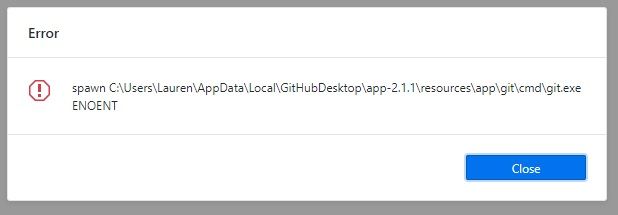
\includegraphics[width=15cm]{github desktop error.jpg}
\end{figure}
\newpage
Objective: Set up static webpage using Github pages\\
Action: Used the command shell instead of Github Desktop.
\newline
\begin{verbatim}
Lauren@Laptop MINGW64 ~ (master)
$ git clone https://github.com/laurenfranks11/laurenfranks11.github.io
Cloning into 'laurenfranks11.github.io'...
remote: Enumerating objects: 3, done.
remote: Counting objects: 100% (3/3), done. 
remote: Total 3 (delta 0), reused 3 (delta 0), pack-reused 0 
Unpacking objects: 100% (3/3), done.

Lauren@Laptop MINGW64 ~ (master)
$ cd laurenfranks11.github.io
\\
Lauren@Laptop MINGW64 ~/laurenfranks11.github.io (master)
$ echo "Hellow World" > index.html
\\
Lauren@Laptop MINGW64 ~/laurenfranks11.github.io (master)
$ git add --all
warning: LF will be replaced by CRLF in index.html.
The file will have its original line endings in your working directory

Lauren@Laptop MINGW64 ~/laurenfranks11.github.io (master)
$ git commit -m "Initial commit"
[master 26e4422] Initial commit
 1 file changed, 1 insertion(+)
 create mode 100644 index.html

Lauren@Laptop MINGW64 ~/laurenfranks11.github.io (master)
$ git push -u origin master
Enumerating objects: 4, done.
Counting objects: 100% (4/4), done.
Delta compression using up to 4 threads
Compressing objects: 100% (2/2), done.
Writing objects: 100% (3/3), 315 bytes | 52.00 KiB/s, done.
Total 3 (delta 0), reused 0 (delta 0)
To https://github.com/laurenfranks11/laurenfranks11.github.io
   c9149a8..26e4422  master -> master
Branch 'master' set up to track remote branch 'master' from 'origin'.
\end{verbatim}

\noindent Result: \href{https://laurenfranks11.github.io./}{https://laurenfranks11.github.io./} successfully created and contains the contents of the html file I created, complete with spelling mistake. 




\end{document}
